\newpage
\maketitle
\begin{center}
\Large \textbf{第7章 隐马可夫模型} \quad 
\end{center}
\begin{abstract}
在本章中我们讲述State Space Model中的隐马可夫模型,并且将该模型用于识别市场所处状态。在下一章中,将以此技术为基础,开发程序化CPA策略。
\end{abstract}
\section{隐马可夫模型}
我们所要研究的金融市场,经常处于变化之中,尤其是受政府政策、宏观调控、业务管制和突发事件等影响,市场状态会发生突然地剧烈的变化,如果我们的策略不作调整,就会使我们遭受巨大的损失。因此,对这种市场机制(Market Regime)进行研究,尤其是识别和预测市场机制的转变,是成功的量化交易所必需的。\newline
我们前几章中对时序信号进行研究过程中,在介绍这些方法时,都在强调这些方法研究的对象是具有平稳性的时序信号。但是当市场机制发生变化时,会使时序信号的均值、方差、自相关性和协方差发生变化,会产生相关性变化、异方差、肥尾等现象,因此研究和预测市场机制变化规律对量化交易而言非常重要。\newline
我们将采用在统计时间序列研究中最重要的隐马可夫模型,来研究市场机制变化规律。这种理论认为,市场机制及其变化,是由内部不可见的过程决定的,其会决定当前的市场机制以及之后市场机制的转换,我们只能通过投资标的的收益率,来间接地观测和研究这一过程。
\subsection{马可夫模型}
马可夫模型是一种随机的状态空间模型,系统会随机的从一种状态切换到另一种状态,状态之间的转换概率只与前一时刻的状态有关,而与之前的状态无关,我们称之为马可夫性质。例如,我们在前面章节中研究的随机游走时间序列,就是一种典型的具有马可夫性质的过程。\newline
根据系统的自治性和系统状态是否完全可见,可以将马可夫模型分为四大类,如下所示:
\begin{table}[H]
\caption{马可夫模型分类}
\label{t000003}
\begin{tabular}{|c|c|c|} \hline
 & 完全可见 & 部分可见 \\ \hline  
自治 & 马可夫链 & 隐马可夫模型(HMM) \\ \hline
控制 & 马可夫决策过程(MDP) & 部分可见马可夫决策过程(POMDP) \\ \hline
\end{tabular}
\end{table}
在这里我们首先明确一个概念,就是系统的状态和观测。系统状态是指系统内部的一种状态,我们不一定能完全观测到。系统观测是我们能够看到的系统性质,是系统状态的间接反映,但是不一定与系统状态相同。这样说比较抽象,让我们来看一个例子,如下图所示:
\begin{figure}[H]
	\caption{系统状态}
	\label{f000066}
	\centering
	
\includegraphics[height=6cm]{images/f000066}
\end{figure}
系统状态就是在远处有一只老虎。但是在有些情况下,我们是无法观测到这个系统状态的,例如下图:
\begin{figure}[H]
	\caption{系统状态和系统观测}
	\label{f000067}
	\centering
	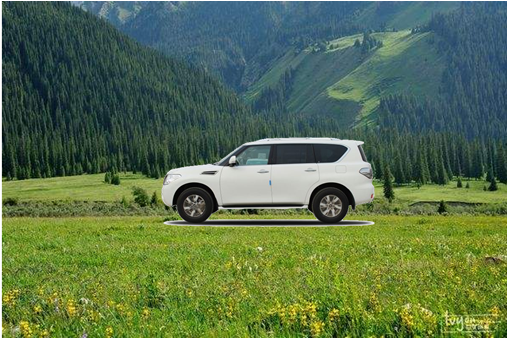
\includegraphics[height=6cm]{images/f000067}
\end{figure}
在上图中,有一辆汽车挡在了老虎的前面,这时我们的观测是系统中有一辆汽车,而我们就无从知道汽车后面还有一只老虎了,因此我们就不能得到系统状态了。在实际应用中,这种状态比较常见,例如在机器人应用中,机器人就观测不到被碍障物遮挡的物体和自己背后的物体,同样在我们的金融应用中,我们也观测不到决定市场机制变化的内部过程。\newline
当系统是自治的,即我们不能改变系统状态,而且系统状态是完全可见的情形,我们称之为马可夫链(MC:Markov Chain)。大家所熟知的马可夫链蒙特卡洛算法,就是在贝叶斯推理计算中一种常用的算法。\newline
当系统还是完体自治的,即我们无法改变系统状态,但是我们只能观测到部分的系统状态,这就是本章将要研究隐马可夫模型。在这种模型中,我们无法直接观测到系统的状态和状态间的转换,我们只能观测系统的某些外在表现,系统内部状态影响系统的外在表现。系统状态具有马可夫属性,即状态间转换只取决于前一状态,与历史状态无关。但是我们对系统的观测,不一定要具有马可夫性质。隐马可夫模型,除了在量化交易领域得到广泛应用外,在语音识别领域也得到了广泛的应用\newline
如果我们即Agent可以通过行动Action来影响系统状态,同时我们可以完全观测到系统的状态,这就是马可夫决策过程(MDP),又称为强化学习(RL:Reinforcement Learning)。这是当前人工智能三大方向之一,前两年大火的Alpha Go/Alpha Zero等,就是基于这种技术。我们会在最后一章中,详细讲解深度强化学习(DRL:Deep Reinforcement Learning)技术在量化交易中的应用。\newline
如果Agent可以通过行动Action来影响系统状态,但是只能间接观测到系统状态的外在表现,这就是部分可见马可夫决策过程(POMDP)。这部分是当前最前沿的研究方向,目前还没有特别成熟有效的解决方案。
\subsection{马可夫模型数学原理}
我们假设有一系列的观察值:$\{ X_{1}, X_{2}, ..., X_{t},...,X_{T} \}$,我们假设我们可以完全观测到系统的状态,因此$X_{t}$同时也是系统状态。同时,我们假设在任意时刻,我们的观测值$X_{t}$包含所有的信息,使我们能够预测出未来系统的状态。这一假设可以表示为如下的概率模型:
\begin{equation}
p(X_{1:T})= p(X_{1})p(X_{2} \vert X_{1})......p(X_{T} \vert X_{T-1})=p(X_{1})\prod_{t=2}^{T} p(X_{t} \vert X_{t-1})
\label{e000082}
\end{equation}
我们将$p(X_{t} \vert X_{t-1})$是$t-1$到$t$时刻的转移函数,同时转移概率与时间无关。\newline
我们假设有K个不同的状态,在$t-1$时刻处于状态$i$,在$t$时刻处于状态$j$,其转移概率为:
\begin{equation}
A_{i,j} = p(X_{t}=j \vert X_{t-1}=i)
\label{e000083}
\end{equation}
为简化问题,我们假设系统仅有两个状态,分别为1和2,在每个时刻,系统都处于这两个状态中的一个,系统从一个状态转移到另一个状态服从概率分布,并且与时间无关,我们可以通过下图来表示:
\begin{figure}[H]
	\caption{状态转移概率图}
	\label{f000068}
	\centering
	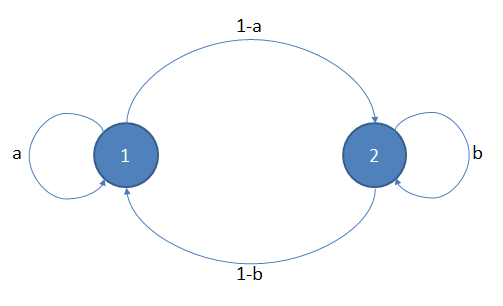
\includegraphics[height=6cm]{images/f000068}
\end{figure}
如图\ref{f000068}所示,当前时刻系统处在状态1,那么下一时刻还是状态1的概率为a,下一时刻为状态2的概率为1-a;如果当前时刻系统处在状态2,那么下一时刻还在状态2的概率为b,转移到状态1的概率为1-b,通常我们可以用状态转移矩阵来表示:
\begin{equation}
A = \begin{bmatrix}
1-\alpha & \alpha \\
\beta & 1 - \beta
\end{bmatrix}
\label{e000084}
\end{equation}
\subsection{隐马可夫模型数学原理}
如果我们不能完全观测到系统的状态,这时我们研究的问题就是隐马可夫模型。以我们本章要研究的问题为例,系统目前的市场机制对我们来说是不可见的,我们只能看到收益率,我们的任务就是根据收益率的变化情况,来推测系统所处的市场机制。\newline
我们假设系统共有K个状态,例如本章所研究的问题,我们可以认为K=3,分别对应为震荡、上涨、下跌,则系统状态用$z_{k},k \in \{1,..., K\}$来表示,系统观测用$x_{t}$来表示,系统状态可以决定系统观测,我们用$p(x_{t} \vert z_{t})$来表示。在隐马可夫模型中,系统处于某一个特定的状态,然后会突然转换到另一个新的状态,这与金融市场通常处于一种行情,突然发生一个突发事件,系统就从一种行情转换到另一种行情,是非常相似的,因此我们用隐马可夫模型来研究这一问题是非常适合的。
从$t=1$到$t=T$时刻,系统状态出现的概率为:
\begin{equation}
p(z_{1:T}) = p(z_{1}) \prod_{t=2}^{T}p(z_{t} \vert z_{t-1})
\label{e000085}
\end{equation}
系统观测出来的概率为:
\begin{equation}
p(x_{1:T} \vert z_{1:T}) = \prod_{t=1}^{T} p(x_{t} \vert z_{t})
\label{e000086}
\end{equation}
则根据观测值推断系统所处状态的概率表示为:
\begin{equation}
p(z_{1:T} \vert x_{1:T}) = p(z_{1:T}) p(x_{1:T} \vert z_{1:T}) = \bigg[ p(z_{1}) \prod_{t=2}^{T}p(z_{t} \vert z_{t-1}) \bigg] \bigg[ \prod_{t=1}^{T} p(x_{t} \vert z_{t}) \bigg]
\label{e000087}
\end{equation}
如果将这个模型应用于我们本章研究的问题,细心的读者可能就会有疑问,在上面的隐马可夫模型中,无论观测值还是系统状态,都是离散变量,而我们的所研究的问题中,股票的收益率为连续值,式\ref{e000087}中的$p(x_{t} \vert z_{t})$怎么计算呢?在实际应用中,我们假设在t时刻系统所处状态为k,即$z_{t}=k$,此时我们可以假设$x_{t}$服从如下所示的高斯分布:
\begin{equation}
x_{t} \sim \mathcal{N}(\mu _{k}, \sigma _{k}^{2})
\label{e000088}
\end{equation}
则有下式成立:
\begin{equation}
p(x_{t} \vert z_{t}=k; \theta) = \mathcal{N} (x_{t} \vert \mu _{k}, \sigma _{k}^{2})
\label{e000089}
\end{equation}
隐马可夫过程可以表示为如下所示形式:
\begin{figure}[H]
	\caption{隐马可夫模型示意图}
	\label{f000069}
	\centering
	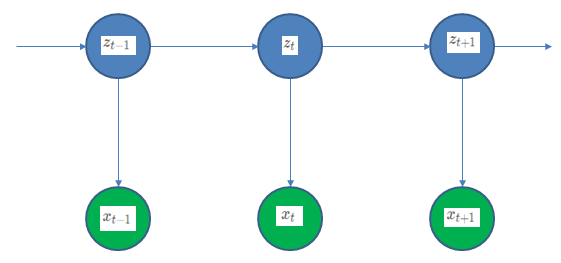
\includegraphics[height=6cm]{images/f000069}
\end{figure}
隐马可夫模型可以实现三大任务:
\begin{itemize}
\item 预测:预测接下来的状态值;
\item 滤波:从观测序列预测当前状态值;
\item 平滑:从观测序列解释过去的状态值;
\end{itemize}
我们本章研究的任务是通过股票收益率变化曲线,预测市场所处状态,因此属于典型的滤波应用。\newline
在介绍了隐马可夫模型的基本理论之后,我们将以工商银行股票为例,讲解基于隐马可夫过程的程序化交易CPA策略。
